\chapter{运动的描述 匀变速直线运动的研究}
\section{描述运动的基本概念}





1.质点1

(1)定义:不考虑物体的大小和形状,把它简化为一个有质量的点,称为“质点”。

(2)质点是一种理想化模型,实际并不存在.

2.参考系

(1)定义: 要描述一个物体的运动,首先要选取某个“其他物体”作参考,观察物体相对于这个“其他物体”的位置是否随时间变化,以及怎样变化。这种用来做参考的物体称为“参考系”。

(2)从理论上来说,参考系的选择是任意的,而如何选择参考系会影响物体的运动状态。。但是,实际在研究地球上的物体的运动的时候,往往以地面为参考系,因为这通常最方便。不过,在解决某些问题时,我们也可以变换参考系,使解决问题更加容易。

3.位移

(1)定义:表示质点的位置变动,它是质点由\_初\_位置指向\_末\_位置的\_有向\_线段.

(2)与路程的区别:位移是\_\_矢\_\_量,路程是\_\_标\_\_量.只有在\_\_单向直线\_\_运动中,位移的大小才等于路程.

4.速度

(1)物理意义:描述物体运动快慢和\_\_运动方向\_\_的物理量,是状态量.

(2)定义式:$v=\dfrac{\Delta x}{\Delta t}$.

(3)大小:在数值上等于单位时间内物体\_\_位移\_\_的大小.

(4)方向:与位移同向,即物体\_\_运动\_\_的方向.

5.平均速度

(1)在变速运动中,物体在某段时间内的\_\_位移\_\_与发生这段位移所用时间的比值叫做这段时间内的平均速度,即$\overline{v}=\dfrac{\Delta x}{\Delta t}$,其方向与\_\_位移\_\_的方向相同.

(2)平均速度反映一段时间内物体运动的平均快慢程度,它与一段时间或一段位移相对应.

6.瞬时速度

(1)运动物体在\_\_某一时刻\_\_(或某一位置)的速度,方向沿轨迹上物体所在点的切线方向指向前进的一侧,是矢量.瞬时速度的大小叫\_\_速率\_\_,是标量.

(2)瞬时速度能精确描述物体运动的快慢,它是在运动时间$\Delta t \rightarrow 0$时的\_\_平均\_\_速度,与某一时刻或某一位置相对应.

(3)平均速率是\_\_路程\_\_与时间的比值,它与平均速度的大小没有对应关系.

7.速度变化量

(1)物理意义:描述物体速度\_\_改变\_\_的物理量,是过程量.

(2)定义式:$\Delta v=v-v_{0}$.

(3)大小:$\Delta v$可以由v与$v_{0}$进行矢量运算得到,也可以由$\Delta v=a \Delta t$计算得到.

(4)方向:可以用矢量图形来描述$\Delta$v的方向,如图甲、乙、丙所示,$\Delta v$的方向由初速度($v_{0}$)矢量的末端指向末速(v)矢量的末端.

\begin{center}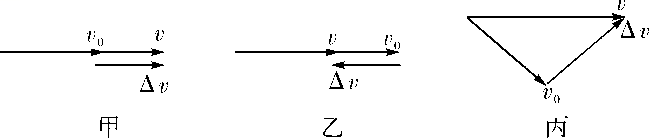
\includegraphics[width=2.94792in,height=0.625in]{media/image5.png}\end{center}
8.加速度

(1)物理意义:描述物体速度\_\_变化快慢和变化方向\_\_的物理量,是状态量.

(2)定义式:$a=\dfrac{\Delta v}{\Delta t}=\dfrac{v-v_{0}}{\Delta t}$.

(3)决定因素:a不是由$v, \Delta t, \Delta v$来决定,而是由F、M来决定.

(4)方向:与$\Delta v$的方向一致,由\_\_合外力\_\_的方向决定,而与$v_{0},v$的方向无关.

\newpage
\subsection{对质点概念的理解}
{[}例1{]}在研究下述运动时,能把物体看做质点的是( B )

A.研究短跑运动员的起跑动作时

B.研究一架无人机的飞行快慢时

C.将一枚硬币用力上抛并猜测它落地时正面是朝上还是朝下时

D.研究汽车在上坡时有无翻倒的危险时
\begin{solution}
	研究短跑运动员的起跑动作、抛出硬币落地时的上下面时,所研究对象的大小和形状不能忽略,故运动员和硬币都不能看做质点;研究汽车翻倒是转动问题,不能将汽车看做质点;研究飞机飞行快慢时,可把飞机看做质点.故选项B正确.
	
	{[}审题突破{]}明确在所研究的问题中,物体的大小和形状是主要因素还是次要因素.
\end{solution}



\begin{center}
\includegraphics[width=0.70833in,height=0.125in]{media/image13.png}

\textbf{建立质点模型的两个关键点}
\end{center}


(1)明确题目中要研究的问题是什么.质点是对实际物体的科学抽象,是研究物体运动时对实际物体进行的近似,真正的质点并不存在.

(2)分析物体的大小和形状对所研究的问题产生的影响能否忽略不计.当物体的大小和形状对所研究运动的影响很小,可以忽略不计时,就可将其视为质点.



\subsection{位移与路程的区别和联系}
\begin{longtable}[]{@{}lll@{}}
\toprule
比较项目 & 位移$x$ & 路程$l$\tabularnewline
\midrule
\endhead
决定因素 & 由始、末位置决定 & 由实际的运动轨迹长度决定\tabularnewline
运算规则 & 矢量的三角形定则或平行四边形定则 &
标量的代数运算\tabularnewline
大小关系 & $x\le l$(路程是位移被无限分割后,所分的各小段位移的绝对值的和)
&\tabularnewline
\bottomrule
\end{longtable}

{[}例2{]}(2017·湖南株洲质检)(多选)关于位移和路程,下列说法正确的是( BD )

A.物体在某一段时间内运动的位移为零,则其一定是静止的

B.物体在某一段时间内运动的路程为零,则其一定是静止的

C.在直线运动中,物体的位移大小一定等于其路程

D.在曲线运动中,物体的位移大小一定小于路程

解析 路程指物体运动轨迹的长度,而位移指由初位置指向末位置的有向线段,只有当物体做单向直线运动时,其位移大小才等于路程.容易判断选项B、D正确,A、C错误.

\newpage
\subsection{平均速度与瞬时速度的区别和联系}

1.两种物体的速度

(1)瞬时速度是运动时间$\Delta t\rightarrow 0$时的平均速度.

(2)对于匀速直线运动,瞬时速度与平均速度相等.

2.关于用平均速度法求瞬时速度

(1)方法概述:由平均速度公式$\bar v=\dfrac{\Delta x}{\Delta t}$可知,当$\Delta x$、$\Delta t$都非常小,趋向于极限时,这时的平均速度就可认为是某一时刻或某一位置的瞬时速度.

(2)选用思路:当已知物体在微小时间$\Delta t$内发生的微小位移$\Delta x$时,可由$\bar v=\dfrac{\Delta x}{\Delta t}$粗略地求出物体在该位置的瞬时速度.

{[}例3{]}(多选)如图所示,物体沿曲线轨迹的箭头方向运动,AB、ABC、ABCD、ABCDE四段曲线轨迹运动所用的时间分别是1
s、2 s、3 s、4 s.下列说法正确的是( ABC )

\begin{center}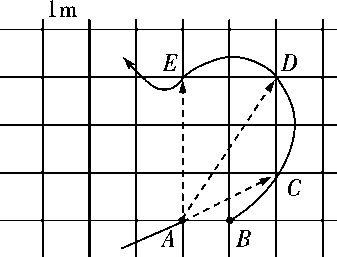
\includegraphics[width=1.53125in,height=1.16667in]{media/image14.png}\end{center}

A.物体在AB段的平均速度大小为1 m/s

B.物体在ABC段的平均速度大小为$\dfrac{\sqrt{5}}{2}$m/s

C.AB段的平均速度比ABC段的平均速度更能反映物体处于A点时的瞬时速度

D.物体在B点的速度等于AC段的平均速度

\begin{solution}
	由$\bar v=\dfrac{\Delta x}{\Delta t}$可得,$\bar v_{AB}=\dfrac{1}{1}m/s=1m/s$,$\bar v_{AC}=\dfrac{\sqrt{5}}{2}m/s$,故选项A、B均正确;所选取的过程离A点越近,其阶段的平均速度越接近A点的瞬时速度,故选项C正确;由A经B到C的过程不是匀变速直线运动过程,故B点虽为AC段的中间时刻,但其速度不等于AC段的平均速度,故选项D错误.
\end{solution}


\begin{center}
\includegraphics[width=0.70833in,height=0.125in]{media/image13.png}

\textbf{平均速度和瞬时速度的三点注意}
\end{center}

(1)求解平均速度必须明确是哪一段位移或哪一段时间内的平均速度.

(2)$\bar v=\dfrac{\Delta x}{\Delta t}$是平均速度的定义式,适用于所有的运动.

(3)用平均速度法近似求解瞬时速度,不仅适用于直线运动,也适用于曲线运动.时间越短,平均速度越接近于瞬时速度.

\newpage
\subsection{速度、速度的变化量和加速度的关系}

1.速度的大小与加速度的大小没有必然联系.

2.速度变化量与加速度没有必然的联系,速度变化量的大小由加速度和速度变化的时间决定.

3.$a=\dfrac{\Delta v}{\Delta t}$是加速度的定义式;加速度的决定式是$a=\dfrac{F}{m}$,即加速度的大小由物体受到的合力F和物体的质量m共同决定,加速度的方向由合力的方向决定.

4.速度增大或减小由速度与加速度的方向关系决定

\begin{center}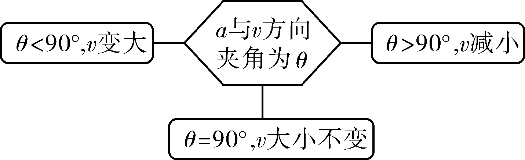
\includegraphics[width=2.38542in,height=0.72917in]{media/image15.png}\end{center}

{[}例4{]}一质点在x轴上运动,初速度$v_0$\textgreater0,加速度a\textgreater0,当加速度a的值由零逐渐增大到某一值后再逐渐减小到零,则该质点( B )

A.速度先增大后减小,直到加速度等于零为止

B.速度一直在增大,直到加速度等于零为止

C.位移先增大,后减小,直到加速度等于零为止

D.位移一直在增大,直到加速度为0为止

\begin{solution}
	由于加速度的方向始终与速度方向相同,质点速度逐渐增大,当加速度减小到零时,速度达到最大值,选项A错误,B正确;位移逐渐增大,当加速度减小到零时,速度不再变化,位移将随时间继续增大,选项C、D错误.
\end{solution}


\begin{center}
\includegraphics[width=0.70833in,height=0.125in]{media/image13.png}

\textbf{对加速度大小和方向的进一步理解}
\end{center}


\begin{center}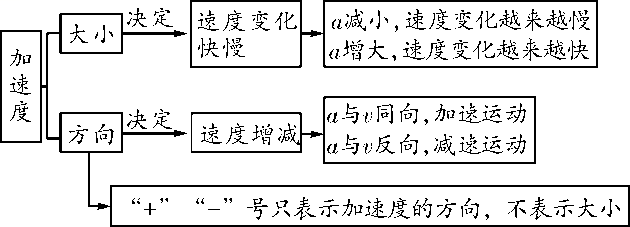
\includegraphics[width=2.86458in,height=1.03125in]{media/image16.png}\end{center}

\newpage
\section{匀变速直线运动的规律及应用}



1.基本规律

(1)速度公式:$v=v_{0}+a t$.

(2)位移公式:$x=v_{0} t+\dfrac{1}{2} a t^2$.

(3)位移速度关系式:$v^{2}-v_{0}^{2}=2 a x$.

这三个基本公式,是解决匀变速直线运动的基石.均为矢量式,应用时应规定正方向.

2.两个重要推论

(1)物体在一段时间内的平均速度等于这段时间中间时刻的瞬时速度,还等于初、末时刻速度矢量和的一半,即$v_{\dfrac{t}{2}}=\dfrac{v_{0}+v}{2}$.

(2)任意两个连续相等的时间间隔T内的位移之差为一恒量,即

$\Delta x=x_{2}-x_{1}=x_{3}-x_{2}=\ldots=x_{n}-x_{n-1}=a T^{2}$.

3.v0=0的四个重要推论

(1)1T末、2T末、3T末\ldots\ldots 瞬时速度的比为

$v_{1} : v_{2} : v_{3} : \ldots : v_{n}=1 : 2 : 3 : \ldots : n$.

(2)1T内、2T内、3T内\ldots\ldots 位移的比为

$x_{1} : x_{2} : x_{3} : \ldots : x_{0}=1^{2} : 2^{2} : 3^{2} : \ldots : n^{2}$.

(3)第一个T内、第二个T内、第三个T内\ldots\ldots 位移的比为

$x_{\mathrm{I}} : x_{\mathrm{II}} : x_{\mathrm{III}} : \ldots : x_{n}=1 : 3 : 5 : \ldots :(2 n-1)$.

(4)从静止开始通过连续相等的位移所用时间的比为

$t_{1} : t_{2} : t_{3} : \ldots : t_{n}=1 :(\sqrt{2}-1) :(\sqrt{3}-\sqrt{2}) : \ldots :(\sqrt{n}-\sqrt{n-1})$.

4.自由落体运动

(1)条件:物体只受\_\_重力\_\_,从\_\_静止\_\_开始下落.

(2)基本规律:

\ding{172}速度公式$v=g t$;

\ding{173}位移公式$h=\dfrac{1}{2} g t^{2}$;

\ding{174}速度位移关系式$v^{2}=2 g h$.

5.竖直上抛运动

(1)运动特点:加速度为g,上升阶段做\_\_匀减速直线\_\_运动,下降阶段做\_\_自由落体\_\_运动.

(2)基本规律:

\ding{172}速度公式$v=v_{0}-g t$;

\ding{173}位移公式$h=v_{0} t-\dfrac{1}{2} g t^{2}$;

\ding{174}速度位移关系式$v^{2}-v_{0}^{2}=-2 g h$.
\newpage
\subsection{匀变速直线运动的规律及应用}

1.运动学公式中正、负号的规定

(1)除时间t外,x、$\mathrm v_0$、v、a均为矢量,所以需要确定正方向,一般以$\mathrm v_0$的方向为正方向.与初速度同向的物理量取正值,反向的物理量取负值,当$\mathrm v_0$=0时,一般以加速度a的方向为正方向.

(2)五个物理量t、$\mathrm v_0$、v、a、x必须针对同一过程.

2.解决匀变速直线运动问题常用的``六法''

\begin{center}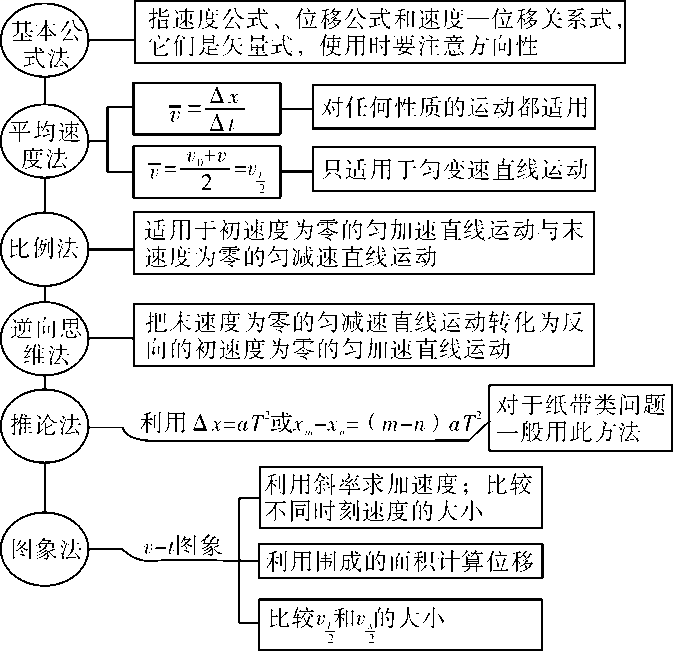
\includegraphics[width=3.06458in,height=2.96319in]{media/image23.png}\end{center}

{[}例1{]}(2017·湖南岳阳检测)如图所示,是冰壶以速度v垂直进入四个宽为l的矩形区域沿虚线做匀减速直线运动,且刚要离开第四个矩形区域的E点时速度恰好为零,冰壶通过前三个矩形的时间为t,试通过所学知识分析并计算冰壶通过第四个矩形所用的时间是多少?(可选用多种方法)

\begin{center}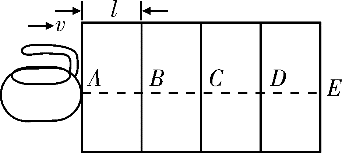
\includegraphics[width=1.55556in,height=0.69444in]{media/image24.png}\end{center}

\begin{solution}
	答案  t
\end{solution}
\begin{center}
\includegraphics[width=0.71319in,height=0.12986in]{media/image25.png}

\textbf{求解匀变速直线运动问题的基本思路}
\end{center}


画过程分析图$\rightarrow$ 判断运动性质$\rightarrow$ 选取正方向$\rightarrow$ 选用公式列方程$\rightarrow$ 解方程并讨论

\newpage
\subsection{自由落体和竖直上抛运动的分析}

{[}例2{]}(2017·山东济南调研)如图所示是一种较精确测量重力加速度g值的方法:将下端装有弹射装置的真空玻璃直管竖直放置,玻璃管足够长,小球竖直向上被弹出,在O点与弹簧分离,然后返回,在O点正上方选取一点P,利用仪器精确测得OP间的距离为H,从O点出发至返回O点的时间间隔为$T_1$,小球两次经过P点的时间间隔为$T_2$.求:

(1)重力加速度g;

(2)若O点距玻璃管底部的距离为$L_0$,求玻璃管最小长度.

\begin{center}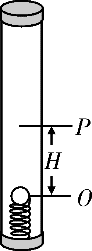
\includegraphics[width=0.41667in,height=1.13889in]{media/image26.png}\end{center}

\begin{solution}
(1)$g=\dfrac{8H}{T_1^2-T_2^2}$ (2)$L_0+\dfrac{T_1^2H}{T_1^2-T_2^2}$

(1)小球从O点上升到最高点有$h_1=\dfrac{1}{2}g(\dfrac{T_1}{2} )^2$,小球从P点上升到最高点有$h_2=\dfrac{1}{2}g(\dfrac{T_2}{2} )^2$,依据题意有$h_1-h_2=H$,联立解得$g=\dfrac{8H}{T_1^2-T_2^2}$.

(2)真空管最小长度$L=L_0+h_1$,解得$L=L_0+\dfrac{T_1^2H}{T_1^2-T_2^2}$.


\end{solution}
\begin{center}
\includegraphics[width=0.71319in,height=0.12986in]{media/image13.png}

\textbf{竖直上抛运动的分析方法}
\end{center}


(1)分段法:可以把竖直上抛运动分成上升阶段的匀减速运动和下降阶段的自由落体运动处理,下降过程是上升过程的逆过程.

(2)整体法:从全过程来看,加速度方向始终与初速度的方向相反,所以也把竖直上抛运动看成是一个匀变速直线运动.
\newpage
\section{运动图象 追及和相遇问题}



1.直线运动的x-t图象

\begin{center}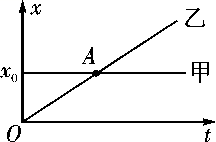
\includegraphics[width=0.97917in,height=0.64583in]{media/image29.png}\end{center}

(1)意义:反映了直线运动的物体\_\_位移\_\_随\_\_时间\_\_变化的规律.

(2)图线上某点切线的斜率的意义

\ding{172}斜率大小:表示物体速度的\_\_大小\_\_.

\ding{173}斜率的正负:表示物体速度的\_\_方向\_\_.

(3)两种特殊的x-t图象

\ding{172}若x-t图象是一条平行于时间轴的直线,说明物体处于\_\_静止\_\_状态.(如图所示甲图线)

\ding{173}若x-t图象是一条倾斜的直线,说明物体在做\_\_匀速直线\_\_运动.(如图所示乙图线)

2.直线运动的v-t图象

\begin{center}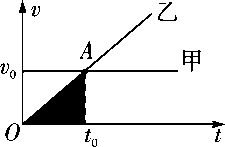
\includegraphics[width=1.02083in,height=0.66667in]{media/image30.png}\end{center}
	

(1)意义:反映了直线运动的物体\_\_速度\_\_随\_\_时间\_\_变化的规律.

(2)图线上某点切线的斜率的意义

\ding{172}斜率的大小:表示物体\_\_加速度\_\_的大小.

\ding{173}斜率的正负:表示物体\_\_加速度\_\_的方向.

(3)两种特殊的v-t图象

\ding{172}匀速直线运动的v-t图象是与横轴\_\_平行\_\_的直线.(如图所示甲图线)

\ding{173}匀变速直线运动的v-t图象是一条\_\_倾斜\_\_的直线.(如图所示乙图线)

(4)图线与坐标轴围成的``面积''的意义

\ding{172}图线与坐标轴围成的``面积''表示相应时间内的\_\_位移\_\_.

\ding{173}若此面积在时间轴的上方,表示这段时间内的位移方向为\_\_正方向\_\_;若此面积在时间轴的下方,表示这段时间内的位移方向为\_\_负方向\_\_.

3.追及和相遇问题

(1)两类追及问题

\ding{172}若后者能追上前者,追上时,两者处于\_\_同一位置\_\_,且后者速度一定不小于前者速度.

\ding{173}若追不上前者,则当后者速度与前者\_\_相等\_\_时,两者相距最近.

(2)两类相遇问题

\ding{172}同向运动的两物体追及,追上时即相遇.

\ding{173}相向运动的物体,当各自发生的位移大小之和等于开始时两物体间的距离时即相遇.

\newpage
\subsection{x-t图象与v-t图象的区别}

\begin{longtable}[]{@{}m{1.5cm}m{6cm}m{6cm}@{}}
\toprule
& x-t图象 & v-t图象\tabularnewline
\midrule
\endhead
轴 & 横轴为时间t,纵轴为位移x & 横轴为时间t,纵轴为速度v\tabularnewline
线 & 倾斜直线表示匀速直线运动 &
倾斜直线表示匀变速直线运动\tabularnewline
斜率 & 表示速度 & 表示加速度\tabularnewline
面积 & 无实际意义 & 图线和时间轴围成的面积表示位移\tabularnewline
纵截距 & 表示初位置 & 表示初速度\tabularnewline
特殊点 & 拐点表示从一种运动变为另一种运动,交点表示相遇 &
拐点表示从一种运动变为另一种运动,交点表示速度相等\tabularnewline
\bottomrule
\end{longtable}

{[}例1{]}(2018·陕西汉中期末)在平直的公路上行驶的a车和b车,其位移——时间图象分别为图中直线a和曲线b,已知b车的加速度恒定且
$ab=-2m/s^2$,当t=3 s时,直线a和曲线b刚好相切,求t=0 s时a车和b车的距离$x_0$.

\begin{center}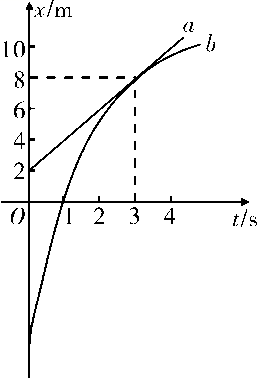
\includegraphics[width=1.16667in,height=1.71875in]{media/image33.png}\end{center}

\begin{solution}
	9 m
\end{solution}
\begin{center}
\includegraphics[width=0.70833in,height=0.125in]{media/image34.png}

\textbf{运动图象中的易错点}
\end{center}


(1)对x-t图象,图线在纵轴上的截距表示t=0时物体的位置,对v-t或a-t图象,图线在纵轴上的截距并不表示t=0时物体的位置.

(2)在v-t图象中,两条图线的交点不表示两物体相遇,而是表示两者速度相同.

(3)两条图线在v轴上的截距不同,不少同学误认为两物体的初始位置不同,位置是否相同应根据题中条件确定.
\newpage
\subsection{追及、相遇问题}

讨论追及、相遇的问题,其实质就是分析讨论两物体在同一时刻能否到达相同的空间位置问题.

1.抓住一个条件,两个关系

(1)一个条件:即两者速度相等,它往往是物体间能否追上、追不上或(两者)距离最大、最小的临界条件,也是分析判断的切入点.

(2)两个关系:即时间关系和位移关系,这两个关系可通过画运动示意图得到.

2.能否追上的判断方法

常见情形:物体A追物体B,开始二者相距$x_0$,则

(1)A追上B时,必有$x_A-x_B=x_0$,且$v_A\ge v_B$.

\begin{center}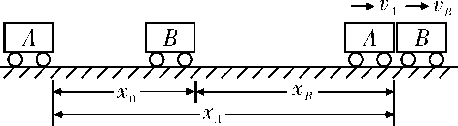
\includegraphics[width=2.08333in,height=0.57292in]{media/image35.png}\end{center}

(2)要使两物体恰好不相撞,必有$x_A-x_B=x_0$,$v_A=v_B$.

{[}例2{]}(2018·江苏镇江模拟)甲、乙两车在同一直线轨道上同向行驶,甲车在前,速度为$v_1=8m/s$,乙车在后,速度为$v_2=16 m/s$,当两车相距$x_0=8m$时,甲车因故开始刹车,加速度大小为$a_1=2m/s^2$,为避免相撞,乙车立即开始刹车,则乙车的加速度至少为多大?
\begin{solution}
	$6m/s^2$
\end{solution}


\begin{center}
\includegraphics[width=0.70833in,height=0.125in]{media/image13.png}

\textbf{追及和相遇问题的求解方法}
\end{center}


(1)解题思路

分析物体运动过程$\rightarrow$画运动示意图$\rightarrow$找两物体位移,时间,速度关系$\rightarrow$ 列位移和速度,时间方程

(2)解题技巧

\ding{172}紧抓``一图三式'',即:过程示意图,时间关系式、速度关系式和位移关系式.

\ding{173}审题应抓住题目中的关键字眼,充分挖掘题目中的隐含条件.如``刚好''\,``恰好''\,``最多''\,``至少''等.往往对应一个临界状态,满足相应的临界条件.

\ding{174}若被追赶的物体做匀减速运动,一定要注意追上前该物体是否已经停止运动,另外还要注意最后对解的讨论分析.
\newpage
